\documentclass{tufte-handout}

%\geometry{showframe}% for debugging purposes -- displays the margins

\usepackage{amsmath}

% Set up the images/graphics package
\usepackage{graphicx}
\setkeys{Gin}{width=\linewidth,totalheight=\textheight,keepaspectratio}
\graphicspath{{graphics/}}

\title{Endocrine Regulation of Macronutrient Homeostasis}
\author{}
\date{}  % if the \date{} command is left out, the current date will be used

% The following package makes prettier tables.  We're all about the bling!
\usepackage{booktabs}

% The units package provides nice, non-stacked fractions and better spacing
% for units.
\usepackage{units}

% The fancyvrb package lets us customize the formatting of verbatim
% environments.  We use a slightly smaller font.
\usepackage{fancyvrb}
\fvset{fontsize=\normalsize}

% Small sections of multiple columns
\usepackage{multicol}

% Provides paragraphs of dummy text
\usepackage{lipsum}

% These commands are used to pretty-print LaTeX commands
\newcommand{\doccmd}[1]{\texttt{\textbackslash#1}}% command name -- adds backslash automatically
\newcommand{\docopt}[1]{\ensuremath{\langle}\textrm{\textit{#1}}\ensuremath{\rangle}}% optional command argument
\newcommand{\docarg}[1]{\textrm{\textit{#1}}}% (required) command argument
\newenvironment{docspec}{\begin{quote}\noindent}{\end{quote}}% command specification environment
\newcommand{\docenv}[1]{\textsf{#1}}% environment name
\newcommand{\docpkg}[1]{\texttt{#1}}% package name
\newcommand{\doccls}[1]{\texttt{#1}}% document class name
\newcommand{\docclsopt}[1]{\texttt{#1}}% document class option name

\begin{document}

\maketitle% this prints the handout title, author, and date

\begin{abstract}
\noindent Metabolism of macronutrients occurs in every cell of the body.  The integrated control of these separate organs is accomplished by endocrine (and neuroendocrine) signaling pathways.  This review material will cover the roles of  key metabolic hormones in normal and patho-physiological states, especially diabetes.  We will cover the endocrine and neuroendocrine regulation of the gastrointestinal system in a separate lecture.  This material should be a review from the endocrine unit in your undergraduate physiology courses, and the course will typically presume these concepts are familiar to you.  For more details about the mechanisms of regulation, such as signal transduction, protein phosphorylation and transcriptional regulation, see the \emph{Metabolic Control Systems} handout, also on Canvas.  If there are concepts or vocabulary in these notes that are unfamiliar to you, please reach out to the instructional team as early as you can so that we can better support your success in this course.
\end{abstract}

\tableofcontents


\pagebreak

\section{Key Terms and Concepts}

Below is a list of some key vocabulary related to this unit.  If any of these terms (or terms not listed here) are unclear or you would like defined, please use the class vocabulary page, available on Canvas.

\begin{description}
	\item [Metabolic Processes]  These are metabolic pathways important to this class.
	\begin{itemize}
		\item Anabolism vs Catabolism
		\item Autophagy
		\item $\beta$ Oxidation
		\item \textit{de novo} Lipogenesis
		\item Gluconeogenesis
		\item Glucose Oxidation, including Glycolysis and the TCA\sidenote{Tricarboxylic Acid Cycle, also known as the Kreb's Cycle or Citric Acid Cycle} Cycle and Oxidative Phosphorylation
		\item Glucose Uptake, including Insulin Stimulated Glucose Uptake
		\item Glycogenesis and Glycogenolysis
		\item Insulin Secretion
		\item Ketogenesis and Ketoacidosis
		\item Lipolysis
		\item Proteolysis
		\item Triglyceride Synthesis
\end{itemize}

	\item[Hormones] You should be familiar with where these hormones come from, and when they are elevated.
	\begin{itemize}
		\item Adrenaline, also known as Epinephrine\sidenote{Along with noradrenaline/norepinephrine}
		\item Cortisol
		\item Glucagon
		\item Growth Hormone
		\item Insulin
		\item Insulin-Like Growth Factor 1 (IGF-1)
	\end{itemize}

	\item [Protein Kinases] These are proteins that phosphorylate other proteins and lead to post-translational regulation\sidenote{A \emph{kinase} is an enzyme that adds a phosphate group to a molecule, a \emph{protein kinase} is an enzyme that adds a phosphate group to another protein.  These reactions are reversed by enzymes called \emph{phosphatases}}.  You should be familiar with what hormones regulate these kinases, and over the course of the semester how they control metabolism.
	\begin{itemize}
		\item Akt\sidenote{Also referred to as Protein Kinase B}
		\item AMP-Activated Protein Kinase (AMPK)
		\item Glycogen Synthase Kinase 3 (GSK3)
		\item Protein Kinase A (PKA)
		\item Mechanistic Target of Rapamycin Complex 1 (mTORC1)
	\end{itemize}
	\item [Transcription Factors].  These regulate gene transcription, or the production of new proteins.  This typically is much slower than allosteric or post-translational regulation.
		\begin{itemize} 
			\item cAMP-Response Element Binding Protein (CREB)
			\item Glucocorticoid Receptor
			\item FOXO\sidenote{A family of Forkhead Box proteins}
			\item Sterol Response Element Binding Protein (SREBP)
		\end{itemize}
\end{description}


\section{Mechanisms of Glucose Regulation}

\newthought{Glucose is typically maintained in a very narrow range}, between 4.4 to 6.1 mmol/L.  The major tissues responsible for regulating glucose levels are listed in Table \ref{glucose-sites}. Glucose levels need to be re-established after changes in feeding status or energy utilization or elevated during the absence of dietary carbohydrates.  In general, when glucose levels decrease, glucagon is released from alpha cells of the pancreas to promote glucose production, either from glycogen breakdown or gluconeogenesis.  Alternately, after a meal when glucose levels increase, insulin is secreted from beta cells of the pancreas causing glucose levels in the blood to decrease.

\begin{margintable}
\caption{Primary sites for regulation of glucose homeostasis}
\label{glucose-sites}
\begin{tabular}{@{}ll@{}}
\textbf{Process }                          & \textbf{Tissue}           \\ \midrule
Insulin Stimulated \\Glucose Uptake & Muscle and Fat   \\ \midrule
Glucose Oxidation & Muscle, Brain \\ \midrule
Glycogen Storage/Release                      & Liver and Muscle   \\ \midrule
Gluconeogenesis & Liver \\ \bottomrule
\end{tabular}
\end{margintable}

For the purposes of the acute maintenance of glucose homeostasis, four organs are the most important; the pancreas, liver, muscle and adipose tissue.  After a meal, muscles are the primary site of glucose disposal \citep{DeFronzo1981}.  The inability to clear glucose from the bloodstream and into muscles is one major cause of the hyperglycemia associated with type 2 diabetes\sidenote{The other proximal cause is unrestrained gluconeogenesis.}.

\newthought{Glucose enters the cell, down a concentration gradient} via passive transport from the blood into most tissues including liver, pancreas, kidneys and the brain.  In these cases the passive transport of glucose into the cell is mostly unregulated.  However, for glucose to enter into muscle and fat tissue, insulin is required.  This is accomplished by moving GLUT4 transporters from intracellular storage sites to the plasma membrane, allowing for glucose influx.  Once inside the cell, insulin will promote both glycogenesis and glycolysis.  

\newthought{Glucose can be stored as glycogen\sidenote{This is known as glycogenesis}}.  To form glycogen, glucose must first be converted through glucose-1-phosphate into UDP-glucose.  This activated form of glucose is then added onto existing glycogen chains through the activity of an enzyme named glycogen synthase.  As we will discuss later in the semester, in addition to being regulated by protein phosphorylation and sub-cellular location, glycogen synthase is also allosterically activated by glucose-6-phosphate, promoting increased glycogen synthesis when glucose levels\sidenote{and therefore G6P levels} in the cell are high.  The combination of the allosteric and post-translational signals mean that when insulin levels are high, glycogenesis is promoted.

\newthought{To liberate glucose from stored glycogen, an enzyme known as glycogen phosphorylase is activated}.  This enzyme hydrolyses glycogen, releasing glucose-1-phosphate, which can then be dephosphorylated into glucose for glycolysis or release into the blood stream.  Hepatic glycogenolysis is the preferred source of short term glucose maintenance.  In addition to post-translational modifications and recruitment to the glycogen pellet by accessory proteins, glycogen phosphorylase is allosterically activated by energy stress such as increases in AMP, or negatively by increases in glucose-6-phosphate levels.  When adrenaline\sidenote{or for the liver, glucagon as well.} is elevated, glycogenolysis occurs releasing stored glucose for energy or to maintain normoglycemia.

\newthought{Gluconeogenesis is the generation of glucose from non-carbohydrate precursor molecules}.  These typically include amino acids, lactate and glycorol\sidenote{Along with free fatty acids, the products of triglyceride breakdown, also known as \emph{lipolysis}.}.  The majority of gluconeogenesis occurs in the liver, and generally is important for glucose production from proteins and lipids after glycogen stores are depleted.  This biochemistry of gluconeogenesis is similar to reversed glycolysis though in several cases different enzymes are used.  As we will discuss later in the lecture, the rate limiting enzymes in gluconeogenesis are phosphoenolpyruvate carboxykinase, fructose-1,6-bisphosphatase and glucose-6-phosphatase.  These enzymes are under both transcriptional and post-translational control as described below.  Both the supply of gluconeogenic precursors (via breakdown of triglycerides and proteins), as well as the activity of gluconeogenic enzymes are reduced by insulin.  Adrenaline and glucagon both \emph{prevent} glycolysis in the liver (but not the muscle).  This is to make sure that the glucose that is produced via gluconeogenesis in liver isn't catabolized back to energy in the liver, but instead is sent to the muscles for uptake and use. Ultimately, the body tries to always ensure that the muscles have sufficient glucose and so it would be counterproductive for adrenaline and glucagon to have a negative regulatory role on muscle glycolysis.

\newthought{When energy is needed}, for example during fasting, the primary source is circulating glucose, followed by the the breakdown of glycogen and then the production of new glucose (gluconeogenesis) from proteins and lipids.  At the same time, the unnecessary synthesis of new glycogen is stopped.  When glucose levels are too high, the first response is uptake and oxidation by the muscle, followed by glycogen synthesis and then eventually by \textit{de novo} lipogenesis.  At this time of excess glucose presence, gluconeogenesis (which is not needed) is stopped.  A summary of how insulin and adrenaline function to control these processes is shown in Table \ref{tab:endocrine-glucose}.

\begin{margintable}
\caption{Primary functions of insulin and the adrenergic hormones, glucagon and adrenaline on glucose homeostasis.}
\label{tab:endocrine-glucose}
\begin{tabular}{@{}lll@{}}
\textbf{Process }                          & \textbf{Insulin}  & \textbf{Adrenergic}           \\ \midrule
Insulin Stimulated \\Glucose Uptake & $\uparrow$ & -  \\ \midrule
Glycolysis - Liver & $\uparrow$ & $\downarrow$ \\  \midrule
Glycolysis - Muscle/Brain & $\uparrow$ & - \\  \midrule
Glycogenolysis & $\downarrow$ & $\uparrow$ \\ \midrule
Gluconeogenesis & $\downarrow$ & $\uparrow$\\ \midrule
Lipolysis & $\downarrow$ & $\uparrow$ \\ \bottomrule

\end{tabular}
\end{margintable}

\section{Pancreatic Cell Types}

In order to balance the energy requirements of all tissues, blood glucose is primarily controlled via endocrine and neuroendocrine mechanisms.  The primary mediators are insulin and glucagon which are secreted from the pancreas during times of hyper and hypoglycemia, respectively.  These two peptide hormones are released from two cell types in the pancreas, the $\alpha$ cells which release glucagon and the $\beta$ cells which release insulin.  Both cell types are located in the Islets of Langerhans within the pancreas (see Figure \ref{pancreas-cells}).

\begin{figure}
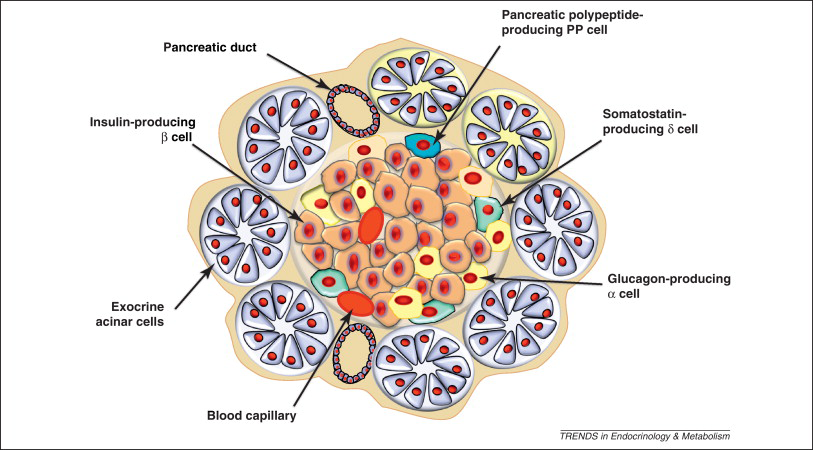
\includegraphics{figures/insulin-cells.png}
\caption{Schematic of a pancreatic islet.  Taken from \citet{Efrat2012}}
\label{pancreas-cells}
\end{figure}

\section{Key Mediators of Insulin Signaling}

Insulin was discovered by Frederick Banting and his colleagues at the University of Toronto in 1921.  They performed experiments in which they injected extracts from pancreas fractions into dogs which had their pancreas surgically removed.  They showed that a secreted substance from the pancreas lowered blood glucose in these dogs \citep{Banting1922b}.  They were then able to confirm that this treatment was also effective in children with type 1 diabetes.  This work led to Banting and John Macleod winning the Nobel Prize in Medicine and Physiology in 1923.  We now know that type 1 diabetes is caused by autoimmune destruction of the pancreatic beta cells\sidenote{At this stage you should be able to predict how the lack of insulin affects glucose disposal, gluconeogenesis, and lipolysis}.  On the other hand, type 2 diabetes, often associated with obesity, is a \emph{peripheral resistance} to the effects of insulin.  This occurs when the muscle, fat tissue and liver stop responding to insulin.

The majority of the actions of insulin are mediated by a protein kinase called Akt (see \citep{Manning2007} for more details).  This protein kinase is activated downstream of both the insulin and IGF1 receptor.  Loss of function mutations in one of the isoforms, \textit{AKT2} in humans results in dramatic peripheral insulin resistance \citep{George2004}\sidenote{These mutations are quite rare in the general population.}.  Akt, once activated by insulin or IGF1 can phosphorylate a variety of proteins including key metabolic enzymes, but also activates key signaling cascades.  Three important cascades we will discuss that function downstream of Akt are FOXO and GSK3 (which are inactivated by Akt) and mTORC1 (which is activated).  

\newthought{The liver is a key central node of metabolism.}  The liver is often the first destination for nutrients that are absorbed in the gut and is a key site of storage and interconversion of nutrients.  For a more detailed review of liver function we recommend the recent review by \citet{Trefts2017}.  Effective liver function is central to many key processes including lipid transport, amino acid oxidation and glucose homeostasis.  In concert with increases in obesity, the prevalence of non-alcoholic fatty liver disease\sidenote{This is often abbreviated as NAFLD.} has been dramatically increasing \citep{Hashimoto2011}.  Impaired liver function renders us less able to interconvert and dispose of macronutrients and less able to detoxify harmful compounds.

\section{Glucagon Promotes Glucose Elevation}

 When glucose levels are low, glucagon is released from alpha cells in the pancreas.  This promotes the breakdown of glycogen stores in liver and muscle, and the generation of glucose from gluconeogenic precursors in the liver.  Glucagon receptors exist mainly in the liver, so glucagon does not exert its main catabolic effects on either adipose or muscle tissue. 

The mechanisms which underlie hypoglycemia induced glucagon release are incompletely understood.  What is clear however, is that when blood glucose levels decrease, glucagon is released from the alpha cells of the pancreas into the portal vein.

\subsection{Glucagon Signal Transduction}

Adrenergic-receptor coupled mediated cAMP synthesis was the first example of a hormonal second messenger.  Earl Sutherland was interested in the regulation of glycogenolysis, and he noticed that if he added adrenaline to intact cells, he could accelerate glycogen breakdown, but if he added it to lysed cells he could not.  In his key experiment he treated one set of livers with adrenaline, then lysed them.  He then added that lysate to a second set of livers which had already been broken.  He found that there was an internal factor (later identified as cAMP) in the stimulated tissues, that could accelerate glycogenolysis in the other tissues \citep{Rall1956}. For this work, Sutherland won the Nobel Prize in Medicine and Physiology in 1971.

In metabolism, the main effector of cAMP in cells is Protein Kinase A (PKA).  This protein kinase is allosterically activated by cAMP and phosphorylates a wide variety of important metabolic substrates.  The identification of PKA and its role in carbohydrate homeostasis led to Fisher and Krebs winning the Nobel Prize in Medicine and Physiology in 1992.  The primary role of glucagon is to increase blood glucose, both by mobilizing glycogen stores and inducing gluconeogenesis.  The mechanisms for this are identical to those for adrenaline, as both of these hormones activate G-protein coupled receptors \sidenote{G protein-coupled receptors are receptors that detect molecules outside the cell and activate internal signals.} and result in PKA activation in the liver.

\subsection{The Primary Target of Glucagon is the Liver}

As described above, glucagon stimulates the breakdown of glycogen.  This proceeds via protein phosphorylation of both glycogen phosphorylase (which activates the enzyme) and glycogen synthase (which inactivates the enzyme).  In combination, this leads to a breakdown of glycogen into glucose.

PKA is the primary mediator of the activation of glycogen phosphorylase.  Once activated by adrenergic signaling, PKA phosphorylates and activates glycogen phosphorylase kinase.  This kinase in turn, phosphorylates and activates glycogen phosphorylase\citep{Krebs1956}.  PKA also directly phosphorylates glycogen synthase, which in concert with the activation of the other glycogen synthase kinases (notably GSK3 and AMPK) leads to increased phosphorylation and inactivation of glycogen synthase.

In addition to the activation of these protein kinases, there is a reduction of glycogen associated protein phosphatase activity.  As a balance, this leads to more highly phosphorylated and therefore more glycogenolytic activities.

\newthought{Glucagon also promotes gluconeogenesis in the liver.}  There are both post-translational and transcriptional mechanisms by which adrenergic signaling promotes gluconeogenesis.  Similar to glycolysis, the allosteric and post-translational regulation of gluconeogenesis is rapid, while the transcriptional regulation is slower but more stable.

Post-translationally, the best studied route by which PKA activates gluconeogenesis is through inactivation of phosphofructokinase-2.  PFK-2 normally generates the carbohydrate Fructose-2,6,-bisphosphate which is a positive regulator of glycolysis and a negative regulator of gluconeogenesis.  The alleviation of this inhibition allows for promotion of the gluconeogenic metabolism.  

Transcriptionally, the transcription factor CREB is phosphorylated by PKA where it plays a role in transcriptionally activating the rate limiting gluconeogenic enzymes PEPCK, FPBase and G6Pase.  This is energetically costly, and occurs slowly.  Transcriptional changes are therefore often more permanent in nature.

\section{Other Glucoregulatory Hormones}

Since glucagon works primarily on liver tissue, different hormonal messengers function to stimulate catabolism of lipid in muscle and fat tissue.  A key difference from adrenaline and glucagon, is that adrenaline also has major effects on fat and muscle tissues, as well as glycogen.  Therefore, in addition to simulating hepatic gluconeogenesis and glycogenolysis, adrenaline also promotes lipid release and muscle glucose oxidation.  Both adrenaline and glucagon function by stimulating adrenergic signaling and cAMP-dependent PKA activation.  Some similarities and differences between glucagon and adrenaline are shown in Table \ref{tab:glucagon-adrenaline}.

\begin{margintable}
\caption{Comparison between glucagon and adrenaline.  Glucagon does not promote lipolysis, think about why that might be the case.}
\label{tab:glucagon-adrenaline}
\begin{tabular}{@{}lll@{}}
 & \textbf{Glucagon}  & \textbf{Adrenaline}           \\ \midrule
Source & Pancreas & Adrenal \\ 
Signal & Hypoglycemia & Acute Stress \\ 
Receptors & Liver & Widespread \\ 
Signaling Pathway & PKA & PKA \\  
Gluconeogenesis & $\uparrow$ & $\uparrow$ \\  
Hepatic Glycolysis & $\downarrow$ & $\downarrow$ \\ 
Lipid Oxidation & $\uparrow$ & $\uparrow$ \\ 
Lipolysis & - & $\uparrow$\\ \bottomrule
\end{tabular}
\end{margintable}

In adipose tissue, adrenaline induces lipolysis, via phosphorylation and activation of Hormone Sensitive Lipase (HSL), Perilipin and Adipocyte Triglyceride Lipase (ATGL).  These proteins function to mobilize triglycerides into free fatty acids for use in other tissues, especially muscle.  For more information on the regulation of lipolysis, see \citep{Young2013}.  At an acute level, these do not contribute much to glucose homeostasis but are extremely important for lipid metabolism.

\newthought{Longer term glucose control is regulated by two other hormones previously discussed, growth hormone and cortisol.}  These hormones are elevated during times of growth or stress where it is important to keep circulating glucose available for other functions.  During a prolonged fast, both GH and cortisol can be released, causing longer-lasting changes which ensure adequate blood supply to the brain.

\newthought{Incretins enhance insulin release}, and are typically released from the gut.  They were first described when it was noted that when equal amounts of glucose are provided either through the gut, or intravenously, the gut-supplied glucose leads to a more robust insulin secretion effect.  Eventually gut-derived peptide hormones, GLP-1 and GIP1\sidenote{glucagon-like peptide 1 and gastric inhibitory peptide respectively} were described.  Both of these peptides are degraded by an enzyme called DPP-4, and inhibitors of this process have provided an exciting new potential therapeutic mechanism for enhancing glucose control.

\section{Pathophysiology Related to Glucose Control}

\subsection{Type I Diabetes Mellitus}

Type I Diabetes is typically caused by autoimmune destruction of pancreatic beta cells.  Without these cells, the pancreas is unable to produce insulin and without careful monitoring and exogenous insulin, blood glucose levels will rise.  At the same time, lipolysis is very high. The excess flow of fatty acids into a liver which is unable to oxidize them\sidenote{We will discuss this in much more detail when we talk about lipid oxidation, but because the liver is diverting TCA cycle intermediates towards gluconeogenesis, the TCA cycle is unable to oxidize Acetyl-CoA.  This results in Acetyl-CoA being converted into a ketone and released from the cell.  The biochemistry is similar to nutritional ketosis, except in that case ketone levels are not typically elevated as high.} results in the production of ketone bodies, which when uncontrolled can lead to diabetic ketoacidosis.

\subsection{Insulin Resistance and Type II Diabetes Mellitus}

Type II diabetes occurs as a result of a multi-step process starting with negative feedback loops on insulin signaling.  As more nutrients are stored, for example in obesity metabolic tissues become resistant to the effects of insulin, likely as a way to protect against excessive lipid storage.  

As tissues become more insulin resistant, more insulin must be secreted by the pancreas to maintain normoglycemia.  If insulin resistance proceeds, more and more insulin will need to be produced and secreted by beta cells.  Eventually the beta cells will be unable to keep up with this demand and glucose levels will rise as the amount of endogenous or exogenous insulin is less and less effective.

\section{Hormonal Regulation of Protein Metabolism}
Protein homeostasis is an important ongoing process that is regulated both at the level of \emph{protein synthesis} and \emph{protein degradation}.  Protein synthesis is especially important in the context of growth and development.  

\subsection{Endocrine Regulators of Protein Synthesis}

There are several hormones that control protein synthesis, often mediated by a protein kinase called mTORC1.   This kinase promotes protein synthesis by increasing the rates of initiation of translation, and the rates of peptide chain elongation.  For more details about how mTORC1 regulates protein production, we recommend this review\citep{Gingras2004}.

\newthought{Insulin and Insulin-like Growth Factor (IGF) are potent activators of protein synthesis}.  Insulin, as described above is secreted by the $\beta$ cells of the pancreas in response to increased blood glucose.  Elevations in amino acids, such as leucine and alanine are also potent activators of insulin secretion \citep{Floyd1966}.  Insulin-like Growth Factor 1, on the other hand is produced in the liver and is regulated both nutritionally, and by Growth Hormone (GH\sidenote{The GH/IGF1 axis will be described in the next section.}).  Both insulin and IGF1\sidenote{There is very little IGF1 activity on adipocytes, so it does not have a strong anti-lipolytic role.} activate receptors in peripheral tissues to promote protein production.   Insulin and IGF1, along with other signals such as elevations in the amino acids Leucine, Lysine or Arginine lead to mTORC1 activation which promotes the synthesis of proteins.

\newthought{Another major regulator of protein synthesis is Growth Hormone}.  Growth hormone is released from the somatotroph cells in the anterior pituitary.  The two primary regulators of GH secretion are the hypothalamic hormones GHRH\sidenote{Growth Hormone Releasing Hormone.} and somatostatin\sidenote{Sometimes called growth hormone inhibiting hormone or GHIH.}.  Growth hormone is highest during youth while people are actively growing.  As a person ages, the amount of growth hormone decreases.  Growth hormone also undergoes a normal diurnal rhythm.  GH levels are highest shortly after going to sleep and lower during the day.  Because of this, most growth occurs during sleeping when nutrients can be used for growth and are not needed for normal activities.  This hormone has two main functions:
\begin{enumerate}
\item Direct actions on bone, muscle, adipocytes and liver tissue via its own receptor\sidenote{In general these functions serve to direct substrates (fatty acids, amino acids and carbohydrates) from storage tissues such as liver and adipose towards growing tissues such as muscle and bone.}.
\item Indirect actions by promoting the release of IGF1 from the liver.  This helps to promote anabolism in muscle and bone.
\end{enumerate}

\subsection{Hormonal Regulators of Protein Degradation}
Protein breakdown occurs via two mechanisms, proteolysis which targets specific proteins for degradation and autophagy\sidenote{or self-eating} which can target entire organelles.  Both of these processes result in the liberation of amino acids from proteins.  Unlike fatty acids (triglycerides) and glucose (glycogen) there is no standard storage molecule for amino acids, so when the body needs amino acids, a variety of proteins are catabolized. 

\newthought{One major pathway by which proteolysis is suppressed is the Insulin/IGF-FOXO pathway}.  Akt-dependent signaling insulin and IGF1 \emph{reduce} FOXO activity (see Figure \ref{fig:foxo-gluconeogenesis}).  When active, FOXO transcriptionally activates proteolytic genes known as atrogenes to liberate amino acids.  These amino acids may be liberated for fuel, or to provide building blocks for gluconeogenesis.  Therefore, when insulin/IGF signaling is active, proteolysis is reduced. 

\begin{marginfigure}
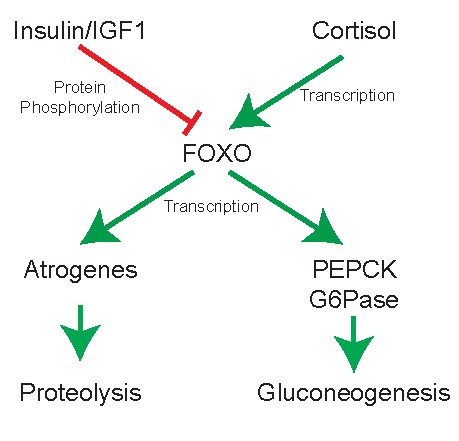
\includegraphics{figures/foxo-gluconeogenesis}
\caption{Schematic of regulation of FOXO and its role in proteolysis and gluconeogenesis.}
\label{fig:foxo-gluconeogenesis}
\end{marginfigure}

\newthought{Cortisol functions to make blood glucose available to key organs such as the brain, during times of stress.}  As such, cortisol promotes gluconeogenesis, by transcriptionally activating several enzymes, including G6Pase, PEPCK and pyruvate carboxylase.  At the same time, cortisol promotes delivery of gluconeogenic precursors such as glycerol (from adipocyte lipolysis), lactate and alanine (from muscle tissue) to the liver.  Chronically elevated cortisol leads to substantial muscle breakdown and is a major side effect of prescribed glucocorticoids or chronic stress.  This is described in Figure \ref{fig:foxo-gluconeogenesis}. Based on this you might be able to make a prediction of how insulin resistance might affect glucose production and proteolysis.

\section{Endocrine Regulation of Lipid Metabolism}

Lipid synthesis is promoted by insulin and reversed by adrenaline.  Triglyceride breakdown can be thought of in two phases, the conversion of triglycerides into fatty acids and glycerol\sidenote{This is known as lipolysis and releases fatty acids and glycerol from stored triglycerides.} and then the conversion of these fatty acids into energy\sidenote{This is known as fatty acid oxidation or $\beta$-oxidation.}.

\newthought{Insulin functions to promote lipid storage} in two ways.  It promotes the production of lipids from precursors\sidenote{This is known as \textit{de novo} lipogenesis.}, promotes the esterifictaion of fatty acids and glycerol into triglycerides and prevents the breakdown of triglycerides into fatty acids.  We will discuss the mechanisms by which insulin controls fat storage later in the semester.

\newthought{To liberate and use lipids for fuel} first, fatty acids are released from adipose tissue, with the activation of $\beta$-oxidation happening concurrently in muscle.  There are several hormones that regulate this, but adrenaline, which promotes both adipocyte lipolysis and muscle lipid oxidation is very important as is the energy sensor AMPK.  As we will learn later in the semester, several key lipolytic and oxidative enzymes are activated by adrenaline (and PKA) mediated protein phosphorylation.

\bibliography{library}
\bibliographystyle{plainnat}

\end{document}
